\documentclass[../../ProjectDocumentation.tex]{subfiles}
%Gummi065=)
\title{\textbf{Display IO Documentation}}
\author{Kyle Lemmon}
\graphicspath{{../display/}}
\date{}

\newcolumntype{C}[1]{>{\centering\let\newline\\\arraybackslash}p{#1}}
\begin{document}

\maketitle

The display I/O consists of three main components: VGA module, Glyph Memory, and Character Set ROM. These three components govern the vga display output.

\subsubsection{VGA Module}
The VGA module is responsible for generating a 640x480, 60Hz, full color VGA signal. This module pulls from both the glyph memory and character set rom in order to compute every pixel in the vga display.



\subsubsection{Glyph Memory}
The glyph memory is accessed as normal program memory, and starts at the address 0xE000. This special memory block is 4800 words long, with each word governing the glyph displayed at that character index. The upper byte of the word specifies the background color and foreground color of the glyph, while the lower byte specifies which character of the character set is displayed. Fig. \ref{fig:glyphmem} shows the binary mapping of a single glyph memory word to the available characters, and the possible colors of that glyph.

\begin{figure}
\begin{tt}
\tiny
\begin{tabular}{|c|c|c|c|c|c|c|c|}
\multicolumn{1}{c}{15} & \multicolumn{1}{c}{14} & \multicolumn{1}{c}{13} & \multicolumn{1}{c}{12} &
\multicolumn{1}{c}{11} & \multicolumn{1}{c}{10} & \multicolumn{1}{c}{9} & \multicolumn{1}{c}{8}  \\
\hline
bg[1] & bg[0] & red[1] & red[0] & grn[1] & grn[0] & blu[1] & blu[0] \\
\hline
\end{tabular}

\begin{tabular}{|c|c|c|c|c|c|c|c|}
\multicolumn{1}{c}{7} & \multicolumn{1}{c}{6} & \multicolumn{1}{c}{5} & \multicolumn{1}{c}{4} &
\multicolumn{1}{c}{3} & \multicolumn{1}{c}{2} & \multicolumn{1}{c}{1} & \multicolumn{1}{c}{0} \\
\hline
chr[7] & chr[6] & chr[5] & chr[4] & chr[3] & chr[2] & chr[1] & chr[0] \\
\hline
\end{tabular}

\end{tt}

\caption{Glyph memory bit map, where bg is the background color, red, grn, and blu are respectively the red, green, and blue foreground color channels, and chr is the character identifier (ACII encoded).}
\label{fig:glyphmem}

\end{figure}



\subsubsection{Character Set ROM}
The character set ROM is non-modifiable and is part of the display module. The character set is similar to ASCII, wherein displayable ASCII characters are mapped to their correct ASCII codes. Non-displayable ASCII characters are remapped to alternate font items in order to have more characters available for display.

The character font is shown in Fig. \ref{fig:charset}. The codes of all characters increase from zero for the upper left 8x8 block, and increase left to right, top to bottom. In that figure, foreground is denoted as white pixels, and the black pixels are the background.

\begin{figure}

\renewcommand{\arraystretch}{1.11}
\begin{tt}
\begin{tabular}{p{0cm} p{0.113cm} p{0.113cm}  p{0.113cm}  p{0.113cm}  p{0.113cm}  p{0.113cm}  p{0.113cm}  p{0.113cm}  p{0.113cm}  p{0.113cm}  p{0.113cm}  p{0.113cm}  p{0.113cm}  p{0.113cm}  p{0.113cm}  p{0.113cm}}

& 0 & 1 & 2 & 3 & 4 & 5 & 6 & 7 & 8 & 9 & A & B & C & D & E & F\\
0 & \multicolumn{16}{c}{\multirow{16}{*}{\raisebox{1cm}{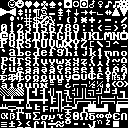
\includegraphics[width=8.43cm]{charset.png}}}} \\
1\\2\\3\\4\\5\\6\\7\\8\\9\\A\\B\\C\\D\\E\\F
\end{tabular}

\end{tt}

\caption{The character set embedded in the processor display module. The character's upper nybble is indicated by the left hex digits, and the lower nybble is indicated by the top column digits. \textbf{Note: If this image appears blurry, you may need to adjust your pdf viewer's settings.} }
\label{fig:charset}

\end{figure}


\end{document}
